

\chapter{动态规划 (2)}


\section{上节课回顾}
上堂课动态规划,我们讲到如果一个大问题可以分解成为小的问题,且有最优子结构的性质,这种时候可以用尝试动态规划。动态规划最简单的例子是矩阵的链式乘法,它是一个序列乘的问题。这个问题的划分可以有很多种,我们不知道怎么分,所以使用枚举。上次我们还讲到单词出错如何进行更改,以及作业查重的方法。这个算法的问题在于需要构造很大的矩阵,比如一篇文章有10K字符,矩阵就是10K*10K这么大,这个空间开销是非常大的。


\section{Hischberg算法}
\subsection{第一个观察}
为了解决这个问题,Hischberg在1975年提出了一个非常精彩的算法,可把空间开销变成$O(m+n)$。该算法核心在三个观察。首先,对于两个字符串,如果只关心最后的分,不需要用到全部的矩阵,只要用到两列就可以。
比如对于下面这个图

\begin{figure}[H]

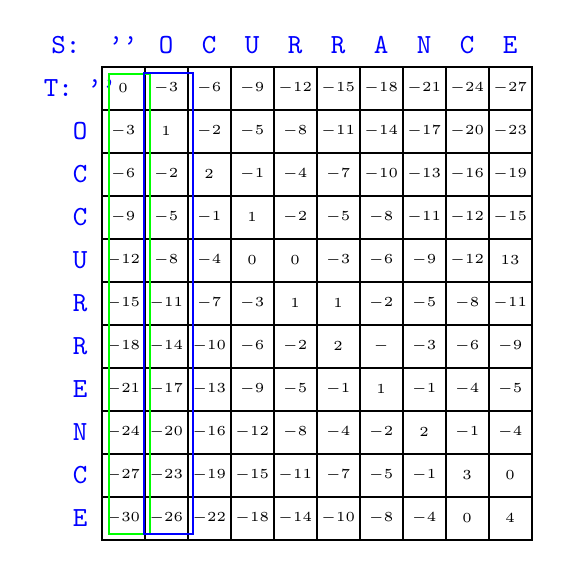
\begin{tikzpicture}[scale=0.78, auto,swap]

  	\def\d{0.7};
	
	%draw index
 \def\dy{1};
 \def\dx{0};

    \foreach \i/\num/\name in {-0.5/\ S:\ /, 1/''/s1,2/O/s2,3/C/s3,4/U/s4,5/R/,6/R/,7/A/,8/N/,9/C/,10/E/}{
           \node[blue,thick] (\name) at (\i*\d+\d/2 + \dx*\d - \d, \d/2 + \dy * \d) {\tt \num};
    }

 \def\dy{0};
 \def\dx{0};
    \foreach \i/\num/\name in { 1/T:\ ''/s1,2/O/s2,3/C/s3,4/C/s4, 5/U/,6/R/,7/R/,8/E/,9/N/,10/C/,11/E/}{
         \node[blue,thick] (\name) at ( -1*\d+\d/2,  0.0 - \i*\d + \d/2 - \dy * \d + \d){\tt  \num};
    }


%score	
 \def\dy{0};
 \def\dx{0};
    \foreach \i/\num/\name in { 0/0/S00,1/-3/S01,2/-6/S2,3/-9/,4/-12/,5/-15/,6/-18/,7/-21/,8/-24/,9/-27/}{
             \draw[  thick ] (\i*\d + \dx*\d,  0+ \dy*\d) rectangle (\i*\d+\d + \dx*\d, \d + \dy*\d);
         \node (\name) at (\i*\d+\d/2 + \dx*\d, \d/2 + \dy*\d) {\tiny $\num$};
    }


 \def\dy{-1};
 \def\dx{0};
    \foreach \i/\num/\name in { 0/-3/,1/1/,2/-2/C,3/-5/LU,4/-8/U,5/-11/,6/-14/,7/-17/,8/-20/,9/-23/}{
             \draw[  thick ] (\i*\d + \dx*\d,  0+ \dy*\d) rectangle (\i*\d+\d + \dx*\d, \d + \dy*\d);
         \node (\name) at (\i*\d+\d/2 + \dx*\d, \d/2 + \dy*\d) {\tiny $\num$};
    }




 \def\dy{-2};
 \def\dx{0};
    \foreach \i/\num/\name in { 0/-6/,1/-2/,2/2/,3/-1/L,4/-4/C,5/-7/,6/-10/,7/-13/,8/-16/,9/-19/}{
             \draw[  thick ] (\i*\d + \dx*\d,  0+ \dy*\d) rectangle (\i*\d+\d + \dx*\d, \d + \dy*\d);
         \node (\name) at (\i*\d+\d/2 + \dx*\d, \d/2 + \dy*\d) {\tiny $\num$};
    }





 \def\dy{-3};
 \def\dx{0};
    \foreach \i/\num/\name in { 0/-9/,1/-5/,2/-1/,3/1/S3,4/-2/,5/-5/,6/-8/,7/-11/,8/-12/,9/-15/}{
             \draw[  thick ] (\i*\d + \dx*\d,  0+ \dy*\d) rectangle (\i*\d+\d + \dx*\d, \d + \dy*\d);
         \node (\name) at (\i*\d+\d/2 + \dx*\d, \d/2 + \dy*\d) {\tiny $\num$};
    }

  \def\dy{-4};
 \def\dx{0};
    \foreach \i/\num/\name in { 0/-12/,1/-8/,2/-4/,3/0/S3,4/0/,5/-3/,6/-6/,7/-9/,8/-12/,9/13/}{
             \draw[  thick ] (\i*\d + \dx*\d,  0+ \dy*\d) rectangle (\i*\d+\d + \dx*\d, \d + \dy*\d);
         \node (\name) at (\i*\d+\d/2 + \dx*\d, \d/2 + \dy*\d) {\tiny $\num$};
    }

  \def\dy{-5};
 \def\dx{0};
    \foreach \i/\num/\name in { 0/-15/,1/-11/,2/-7/,3/-3/S3,4/1/,5/1/,6/-2/,7/-5/,8/-8/,9/-11/}{
             \draw[  thick ] (\i*\d + \dx*\d,  0+ \dy*\d) rectangle (\i*\d+\d + \dx*\d, \d + \dy*\d);
         \node (\name) at (\i*\d+\d/2 + \dx*\d, \d/2 + \dy*\d) {\tiny $\num$};
    }

  \def\dy{-6};
 \def\dx{0};
    \foreach \i/\num/\name in { 0/-18/,1/-14/,2/-10/,3/-6/S3,4/-2/,5/2/,6/-/,7/-3/,8/-6/,9/-9/}{
             \draw[  thick ] (\i*\d + \dx*\d,  0+ \dy*\d) rectangle (\i*\d+\d + \dx*\d, \d + \dy*\d);
         \node (\name) at (\i*\d+\d/2 + \dx*\d, \d/2 + \dy*\d) {\tiny $\num$};
    }

  \def\dy{-7};
 \def\dx{0};
    \foreach \i/\num/\name in { 0/-21/,1/-17/,2/-13/,3/-9/S3,4/-5/,5/-1/,6/1/,7/-1/,8/-4/,9/-5/}{
             \draw[  thick ] (\i*\d + \dx*\d,  0+ \dy*\d) rectangle (\i*\d+\d + \dx*\d, \d + \dy*\d);
         \node (\name) at (\i*\d+\d/2 + \dx*\d, \d/2 + \dy*\d) {\tiny $\num$};
    }

  \def\dy{-8};
 \def\dx{0};
    \foreach \i/\num/\name in { 0/-24/,1/-20/,2/-16/,3/-12/S3,4/-8/,5/-4/,6/-2/,7/2/,8/-1/,9/-4/}{
             \draw[  thick ] (\i*\d + \dx*\d,  0+ \dy*\d) rectangle (\i*\d+\d + \dx*\d, \d + \dy*\d);
         \node (\name) at (\i*\d+\d/2 + \dx*\d, \d/2 + \dy*\d) {\tiny $\num$};
    }

  \def\dy{-9};
 \def\dx{0};
    \foreach \i/\num/\name in { 0/-27/,1/-23/,2/-19/,3/-15/S3,4/-11/,5/-7/,6/-5/,7/-1/,8/3/LU,9/0/U}{
             \draw[  thick ] (\i*\d + \dx*\d,  0+ \dy*\d) rectangle (\i*\d+\d + \dx*\d, \d + \dy*\d);
         \node (\name) at (\i*\d+\d/2 + \dx*\d, \d/2 + \dy*\d) {\tiny $\num$};
    }

  \def\dy{-10};
 \def\dx{0};
    \foreach \i/\num/\name in { 0/-30/Sn0,1/-26/Sn1,2/-22/,3/-18/S3,4/-14/,5/-10/,6/-8/,7/-4/,8/0/L,9/4/C}{
             \draw[  thick ] (\i*\d + \dx*\d,  0+ \dy*\d) rectangle (\i*\d+\d + \dx*\d, \d + \dy*\d);
         \node (\name) at (\i*\d+\d/2 + \dx*\d, \d/2 + \dy*\d) {\tiny $\num$};
    }


    \draw[green, thick] (S00.north west) rectangle (Sn0.south east);
     \draw[blue, thick] (S01.north west) rectangle (Sn1.south east);


\end{tikzpicture}
\end{figure}     

我通过初始化知道了最左边一列的分,然后下一列的分怎么算? 我们知道任意一个单元的分依赖于临近的三个单元。所以,知道第一列以后,我们可以算出第二列。这时候,我只需要放弃第一列空间,计算第三列,以此类推,我们只是依赖了两个数组,就可以计算到最后的分。下面的图展现了计算过程。
\begin{figure}[H]

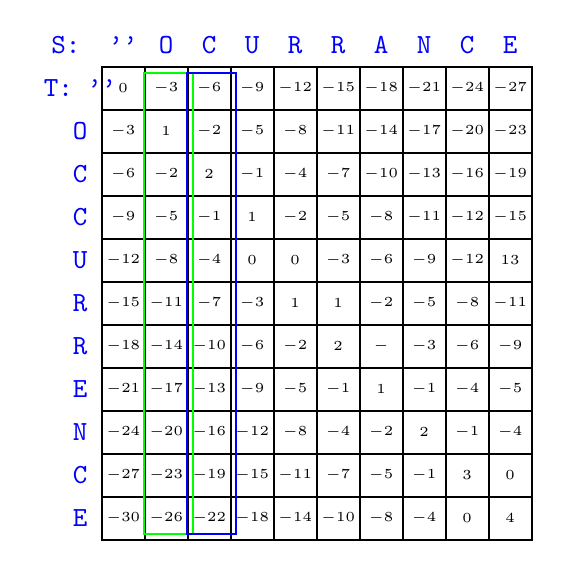
\begin{tikzpicture}[scale=0.78, auto,swap]

  	\def\d{0.7};
	
	%draw index
 \def\dy{1};
 \def\dx{0};

    \foreach \i/\num/\name in {-0.5/\ S:\ /, 1/''/s1,2/O/s2,3/C/s3,4/U/s4,5/R/,6/R/,7/A/,8/N/,9/C/,10/E/}{
           \node[blue,thick] (\name) at (\i*\d+\d/2 + \dx*\d - \d, \d/2 + \dy * \d) {\tt \num};
    }

 \def\dy{0};
 \def\dx{0};
    \foreach \i/\num/\name in { 1/T:\ ''/s1,2/O/s2,3/C/s3,4/C/s4, 5/U/,6/R/,7/R/,8/E/,9/N/,10/C/,11/E/}{
         \node[blue,thick] (\name) at ( -1*\d+\d/2,  0.0 - \i*\d + \d/2 - \dy * \d + \d){\tt  \num};
    }


%score	
 \def\dy{0};
 \def\dx{0};
    \foreach \i/\num/\name in { 0/0/S00,1/-3/S01,2/-6/S02,3/-9/,4/-12/,5/-15/,6/-18/,7/-21/,8/-24/,9/-27/}{
             \draw[  thick ] (\i*\d + \dx*\d,  0+ \dy*\d) rectangle (\i*\d+\d + \dx*\d, \d + \dy*\d);
         \node (\name) at (\i*\d+\d/2 + \dx*\d, \d/2 + \dy*\d) {\tiny $\num$};
    }


 \def\dy{-1};
 \def\dx{0};
    \foreach \i/\num/\name in { 0/-3/,1/1/,2/-2/C,3/-5/LU,4/-8/U,5/-11/,6/-14/,7/-17/,8/-20/,9/-23/}{
             \draw[  thick ] (\i*\d + \dx*\d,  0+ \dy*\d) rectangle (\i*\d+\d + \dx*\d, \d + \dy*\d);
         \node (\name) at (\i*\d+\d/2 + \dx*\d, \d/2 + \dy*\d) {\tiny $\num$};
    }




 \def\dy{-2};
 \def\dx{0};
    \foreach \i/\num/\name in { 0/-6/,1/-2/,2/2/,3/-1/L,4/-4/C,5/-7/,6/-10/,7/-13/,8/-16/,9/-19/}{
             \draw[  thick ] (\i*\d + \dx*\d,  0+ \dy*\d) rectangle (\i*\d+\d + \dx*\d, \d + \dy*\d);
         \node (\name) at (\i*\d+\d/2 + \dx*\d, \d/2 + \dy*\d) {\tiny $\num$};
    }





 \def\dy{-3};
 \def\dx{0};
    \foreach \i/\num/\name in { 0/-9/,1/-5/,2/-1/,3/1/S3,4/-2/,5/-5/,6/-8/,7/-11/,8/-12/,9/-15/}{
             \draw[  thick ] (\i*\d + \dx*\d,  0+ \dy*\d) rectangle (\i*\d+\d + \dx*\d, \d + \dy*\d);
         \node (\name) at (\i*\d+\d/2 + \dx*\d, \d/2 + \dy*\d) {\tiny $\num$};
    }

  \def\dy{-4};
 \def\dx{0};
    \foreach \i/\num/\name in { 0/-12/,1/-8/,2/-4/,3/0/S3,4/0/,5/-3/,6/-6/,7/-9/,8/-12/,9/13/}{
             \draw[  thick ] (\i*\d + \dx*\d,  0+ \dy*\d) rectangle (\i*\d+\d + \dx*\d, \d + \dy*\d);
         \node (\name) at (\i*\d+\d/2 + \dx*\d, \d/2 + \dy*\d) {\tiny $\num$};
    }

  \def\dy{-5};
 \def\dx{0};
    \foreach \i/\num/\name in { 0/-15/,1/-11/,2/-7/,3/-3/S3,4/1/,5/1/,6/-2/,7/-5/,8/-8/,9/-11/}{
             \draw[  thick ] (\i*\d + \dx*\d,  0+ \dy*\d) rectangle (\i*\d+\d + \dx*\d, \d + \dy*\d);
         \node (\name) at (\i*\d+\d/2 + \dx*\d, \d/2 + \dy*\d) {\tiny $\num$};
    }

  \def\dy{-6};
 \def\dx{0};
    \foreach \i/\num/\name in { 0/-18/,1/-14/,2/-10/,3/-6/S3,4/-2/,5/2/,6/-/,7/-3/,8/-6/,9/-9/}{
             \draw[  thick ] (\i*\d + \dx*\d,  0+ \dy*\d) rectangle (\i*\d+\d + \dx*\d, \d + \dy*\d);
         \node (\name) at (\i*\d+\d/2 + \dx*\d, \d/2 + \dy*\d) {\tiny $\num$};
    }

  \def\dy{-7};
 \def\dx{0};
    \foreach \i/\num/\name in { 0/-21/,1/-17/,2/-13/,3/-9/S3,4/-5/,5/-1/,6/1/,7/-1/,8/-4/,9/-5/}{
             \draw[  thick ] (\i*\d + \dx*\d,  0+ \dy*\d) rectangle (\i*\d+\d + \dx*\d, \d + \dy*\d);
         \node (\name) at (\i*\d+\d/2 + \dx*\d, \d/2 + \dy*\d) {\tiny $\num$};
    }

  \def\dy{-8};
 \def\dx{0};
    \foreach \i/\num/\name in { 0/-24/,1/-20/,2/-16/,3/-12/S3,4/-8/,5/-4/,6/-2/,7/2/,8/-1/,9/-4/}{
             \draw[  thick ] (\i*\d + \dx*\d,  0+ \dy*\d) rectangle (\i*\d+\d + \dx*\d, \d + \dy*\d);
         \node (\name) at (\i*\d+\d/2 + \dx*\d, \d/2 + \dy*\d) {\tiny $\num$};
    }

  \def\dy{-9};
 \def\dx{0};
    \foreach \i/\num/\name in { 0/-27/,1/-23/,2/-19/,3/-15/S3,4/-11/,5/-7/,6/-5/,7/-1/,8/3/LU,9/0/U}{
             \draw[  thick ] (\i*\d + \dx*\d,  0+ \dy*\d) rectangle (\i*\d+\d + \dx*\d, \d + \dy*\d);
         \node (\name) at (\i*\d+\d/2 + \dx*\d, \d/2 + \dy*\d) {\tiny $\num$};
    }

  \def\dy{-10};
 \def\dx{0};
    \foreach \i/\num/\name in { 0/-30/Sn0,1/-26/Sn1,2/-22/Sn2,3/-18/S3,4/-14/,5/-10/,6/-8/,7/-4/,8/0/L,9/4/C}{
             \draw[  thick ] (\i*\d + \dx*\d,  0+ \dy*\d) rectangle (\i*\d+\d + \dx*\d, \d + \dy*\d);
         \node (\name) at (\i*\d+\d/2 + \dx*\d, \d/2 + \dy*\d) {\tiny $\num$};
    }


    \draw[green, thick] (S01.north west) rectangle (Sn1.south east);
     \draw[blue, thick] (S02.north west) rectangle (Sn2.south east);


\end{tikzpicture}
\end{figure}    
\begin{figure}[H]

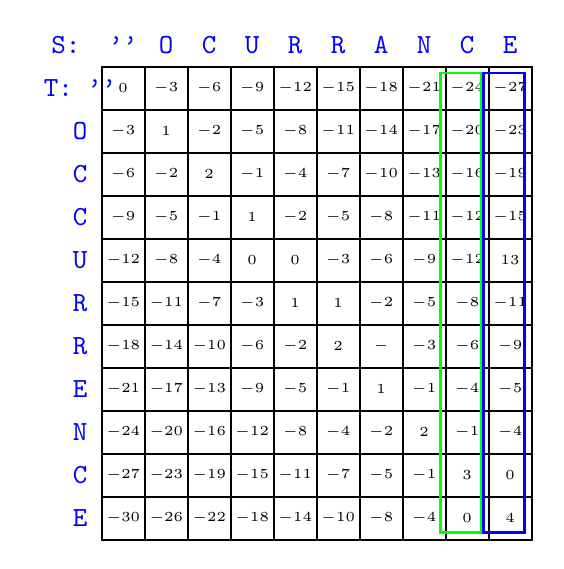
\begin{tikzpicture}[scale=0.78, auto,swap]

  	\def\d{0.7};
	
	%draw index
 \def\dy{1};
 \def\dx{0};

    \foreach \i/\num/\name in {-0.5/\ S:\ /, 1/''/s1,2/O/s2,3/C/s3,4/U/s4,5/R/,6/R/,7/A/,8/N/,9/C/,10/E/}{
           \node[blue,thick] (\name) at (\i*\d+\d/2 + \dx*\d - \d, \d/2 + \dy * \d) {\tt \num};
    }

 \def\dy{0};
 \def\dx{0};
    \foreach \i/\num/\name in { 1/T:\ ''/s1,2/O/s2,3/C/s3,4/C/s4, 5/U/,6/R/,7/R/,8/E/,9/N/,10/C/,11/E/}{
         \node[blue,thick] (\name) at ( -1*\d+\d/2,  0.0 - \i*\d + \d/2 - \dy * \d + \d){\tt  \num};
    }


%score	
 \def\dy{0};
 \def\dx{0};
    \foreach \i/\num/\name in { 0/0/S00,1/-3/S01,2/-6/S2,3/-9/,4/-12/,5/-15/,6/-18/,7/-21/,8/-24/S0n1,9/-27/S0n}{
             \draw[  thick ] (\i*\d + \dx*\d,  0+ \dy*\d) rectangle (\i*\d+\d + \dx*\d, \d + \dy*\d);
         \node (\name) at (\i*\d+\d/2 + \dx*\d, \d/2 + \dy*\d) {\tiny $\num$};
    }


 \def\dy{-1};
 \def\dx{0};
    \foreach \i/\num/\name in { 0/-3/,1/1/,2/-2/C,3/-5/LU,4/-8/U,5/-11/,6/-14/,7/-17/,8/-20/,9/-23/}{
             \draw[  thick ] (\i*\d + \dx*\d,  0+ \dy*\d) rectangle (\i*\d+\d + \dx*\d, \d + \dy*\d);
         \node (\name) at (\i*\d+\d/2 + \dx*\d, \d/2 + \dy*\d) {\tiny $\num$};
    }




 \def\dy{-2};
 \def\dx{0};
    \foreach \i/\num/\name in { 0/-6/,1/-2/,2/2/,3/-1/L,4/-4/C,5/-7/,6/-10/,7/-13/,8/-16/,9/-19/}{
             \draw[  thick ] (\i*\d + \dx*\d,  0+ \dy*\d) rectangle (\i*\d+\d + \dx*\d, \d + \dy*\d);
         \node (\name) at (\i*\d+\d/2 + \dx*\d, \d/2 + \dy*\d) {\tiny $\num$};
    }





 \def\dy{-3};
 \def\dx{0};
    \foreach \i/\num/\name in { 0/-9/,1/-5/,2/-1/,3/1/S3,4/-2/,5/-5/,6/-8/,7/-11/,8/-12/,9/-15/}{
             \draw[  thick ] (\i*\d + \dx*\d,  0+ \dy*\d) rectangle (\i*\d+\d + \dx*\d, \d + \dy*\d);
         \node (\name) at (\i*\d+\d/2 + \dx*\d, \d/2 + \dy*\d) {\tiny $\num$};
    }

  \def\dy{-4};
 \def\dx{0};
    \foreach \i/\num/\name in { 0/-12/,1/-8/,2/-4/,3/0/S3,4/0/,5/-3/,6/-6/,7/-9/,8/-12/,9/13/}{
             \draw[  thick ] (\i*\d + \dx*\d,  0+ \dy*\d) rectangle (\i*\d+\d + \dx*\d, \d + \dy*\d);
         \node (\name) at (\i*\d+\d/2 + \dx*\d, \d/2 + \dy*\d) {\tiny $\num$};
    }

  \def\dy{-5};
 \def\dx{0};
    \foreach \i/\num/\name in { 0/-15/,1/-11/,2/-7/,3/-3/S3,4/1/,5/1/,6/-2/,7/-5/,8/-8/,9/-11/}{
             \draw[  thick ] (\i*\d + \dx*\d,  0+ \dy*\d) rectangle (\i*\d+\d + \dx*\d, \d + \dy*\d);
         \node (\name) at (\i*\d+\d/2 + \dx*\d, \d/2 + \dy*\d) {\tiny $\num$};
    }

  \def\dy{-6};
 \def\dx{0};
    \foreach \i/\num/\name in { 0/-18/,1/-14/,2/-10/,3/-6/S3,4/-2/,5/2/,6/-/,7/-3/,8/-6/,9/-9/}{
             \draw[  thick ] (\i*\d + \dx*\d,  0+ \dy*\d) rectangle (\i*\d+\d + \dx*\d, \d + \dy*\d);
         \node (\name) at (\i*\d+\d/2 + \dx*\d, \d/2 + \dy*\d) {\tiny $\num$};
    }

  \def\dy{-7};
 \def\dx{0};
    \foreach \i/\num/\name in { 0/-21/,1/-17/,2/-13/,3/-9/S3,4/-5/,5/-1/,6/1/,7/-1/,8/-4/,9/-5/}{
             \draw[  thick ] (\i*\d + \dx*\d,  0+ \dy*\d) rectangle (\i*\d+\d + \dx*\d, \d + \dy*\d);
         \node (\name) at (\i*\d+\d/2 + \dx*\d, \d/2 + \dy*\d) {\tiny $\num$};
    }

  \def\dy{-8};
 \def\dx{0};
    \foreach \i/\num/\name in { 0/-24/,1/-20/,2/-16/,3/-12/S3,4/-8/,5/-4/,6/-2/,7/2/,8/-1/,9/-4/}{
             \draw[  thick ] (\i*\d + \dx*\d,  0+ \dy*\d) rectangle (\i*\d+\d + \dx*\d, \d + \dy*\d);
         \node (\name) at (\i*\d+\d/2 + \dx*\d, \d/2 + \dy*\d) {\tiny $\num$};
    }

  \def\dy{-9};
 \def\dx{0};
    \foreach \i/\num/\name in { 0/-27/,1/-23/,2/-19/,3/-15/S3,4/-11/,5/-7/,6/-5/,7/-1/,8/3/LU,9/0/U}{
             \draw[  thick ] (\i*\d + \dx*\d,  0+ \dy*\d) rectangle (\i*\d+\d + \dx*\d, \d + \dy*\d);
         \node (\name) at (\i*\d+\d/2 + \dx*\d, \d/2 + \dy*\d) {\tiny $\num$};
    }

  \def\dy{-10};
 \def\dx{0};
    \foreach \i/\num/\name in { 0/-30/Sn0,1/-26/Sn1,2/-22/,3/-18/S3,4/-14/,5/-10/,6/-8/,7/-4/,8/0/Snn1,9/4/Snn}{
             \draw[  thick ] (\i*\d + \dx*\d,  0+ \dy*\d) rectangle (\i*\d+\d + \dx*\d, \d + \dy*\d);
         \node (\name) at (\i*\d+\d/2 + \dx*\d, \d/2 + \dy*\d) {\tiny $\num$};
    }


    \draw[green, thick] (S0n1.north west) rectangle (Snn1.south east);
     \draw[blue, thick] (S0n.north west) rectangle (Snn.south east);


\end{tikzpicture}
\end{figure}     

对于上面的观察,我们可以写一个算法计算最后的分

\sc Prefix\_Space\_Efficient\_Alignment( S, T, score )
\begin{algorithmic}[1]
\FOR {$i=0$ to $m$ }
\STATE $score[i] = -3*i;$
\ENDFOR
\FOR {$i=1$ to $m$  }
\FOR {$j=1$ to $n$  }
\STATE $newscore[j] = \max \{score[j-1] + \delta(S_i,T_j), score[j] - 3, newscore[j-1] - 3\};$
\ENDFOR
\STATE $newscore[0] = 0;$
\FOR {$j=1$ to $n$  }
\STATE $score[j] = newscore[j];$
\ENDFOR
\ENDFOR
\RETURN {$score[n]$ };
\end{algorithmic}

\subsection{第二个观察}

我们刚才做的算法,是从左往右的,都是S的前缀和T的前缀进行计算。但是其实也是可以S的后缀进行计算。一开始我问的是,S的最后一个字符E 是怎么来的。我们定义的子问题用到了S的前缀和T 的前缀。当基于S和T的后缀定义子问题的时候,我们问的是:S 的第一个字符是怎么来的?这也会有三种情况。这样子问题,就变成S和T的后缀的最优连配。这时候,矩阵要变成从下往上,从右往左开始算。算到最后我们发现分数是一样的,也是4。
\begin{figure}[H]

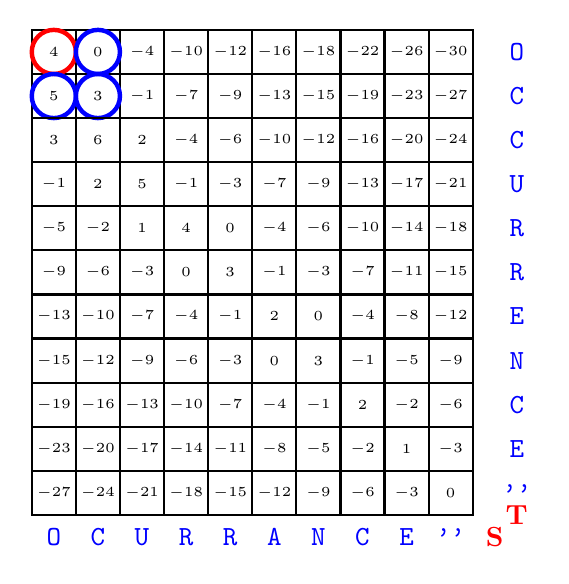
\begin{tikzpicture}[scale=0.8, auto,swap]

  	\def\d{0.7};
	
	%draw index
 \def\dy{-11};
 \def\dx{0};

    \foreach \i/\num/\name in {  11/S/}{
           \node[red,ultra thick] (\name) at (\i*\d+\d/2 + \dx*\d - \d, \d/2 + \dy * \d) {\bf \num};
    }

    \foreach \i/\num/\name in {   10/''/s1, 1/O/s2,2/C/s3,3/U/s4,4/R/,5/R/,6/A/,7/N/,8/C/,9/E/}{
           \node[blue,thick] (\name) at (\i*\d+\d/2 + \dx*\d - \d, \d/2 + \dy * \d) {\tt \num};
    }

 \def\dy{0};
 \def\dx{10.5};
    \foreach \i/\num/\name in {  11/''/s1,1/O/s2,2/C/s3,3/C/s4, 4/U/,5/R/,6/R/,7/E/,8/N/,9/C/,10/E/}{
         \node[blue,thick] (\name) at (\dx*\d+\d/2,  0.0 - \i*\d + \d/2 - \dy * \d + \d){\tt  \num};
    }
    \foreach \i/\num/\name in { 11.5/T/}{
             \node[red,ultra thick] (\name) at (\dx*\d+\d/2,  0.0 - \i*\d + \d/2 - \dy * \d + \d){\bf  \num};
    }

%score	
 \def\dy{0};
 \def\dx{0};
    \foreach \i/\num/\name in { 0/4/C,1/0/S1,2/-4/,3/-10/,4/-12/,5/-16/,6/-18/,7/-22/,8/-26/,9/-30/}{
             \draw[  thick ] (\i*\d + \dx*\d,  0+ \dy*\d) rectangle (\i*\d+\d + \dx*\d, \d + \dy*\d);
         \node (\name) at (\i*\d+\d/2 + \dx*\d, \d/2 + \dy*\d) {\tiny $\num$};
    }


 \def\dy{-1};
 \def\dx{0};
    \foreach \i/\num/\name in { 0/5/S2,1/3/L,2/-1/,3/-7/,4/-9/,5/-13/,6/-15/,7/-19/,8/-23/,9/-27/}{
             \draw[  thick ] (\i*\d + \dx*\d,  0+ \dy*\d) rectangle (\i*\d+\d + \dx*\d, \d + \dy*\d);
         \node (\name) at (\i*\d+\d/2 + \dx*\d, \d/2 + \dy*\d) {\tiny $\num$};
    }

    \draw[red,ultra thick] (C) circle[radius=\d/2];
   \draw[blue,ultra thick] (S1) circle[radius=\d/2];
   \draw[blue,ultra thick] (S2) circle[radius=\d/2];
   \draw[blue,ultra thick] (L) circle[radius=\d/2];



 \def\dy{-2};
 \def\dx{0};
    \foreach \i/\num/\name in { 0/3/,1/6/,2/2/,3/-4/S3,4/-6/,5/-10/,6/-12/,7/-16/,8/-20/,9/-24/}{
             \draw[  thick ] (\i*\d + \dx*\d,  0+ \dy*\d) rectangle (\i*\d+\d + \dx*\d, \d + \dy*\d);
         \node (\name) at (\i*\d+\d/2 + \dx*\d, \d/2 + \dy*\d) {\tiny $\num$};
    }

 \def\dy{-3};
 \def\dx{0};
    \foreach \i/\num/\name in { 0/-1/,1/2/,2/5/,3/-1/S3,4/-3/,5/-7/,6/-9/,7/-13/,8/-17/,9/-21/}{
             \draw[  thick ] (\i*\d + \dx*\d,  0+ \dy*\d) rectangle (\i*\d+\d + \dx*\d, \d + \dy*\d);
         \node (\name) at (\i*\d+\d/2 + \dx*\d, \d/2 + \dy*\d) {\tiny $\num$};
    }

  \def\dy{-4};
 \def\dx{0};
    \foreach \i/\num/\name in { 0/-5/,1/-2/,2/1/,3/4/S3,4/0/,5/-4/,6/-6/,7/-10/,8/-14/,9/-18/}{
             \draw[  thick ] (\i*\d + \dx*\d,  0+ \dy*\d) rectangle (\i*\d+\d + \dx*\d, \d + \dy*\d);
         \node (\name) at (\i*\d+\d/2 + \dx*\d, \d/2 + \dy*\d) {\tiny $\num$};
    }

  \def\dy{-5};
 \def\dx{0};
    \foreach \i/\num/\name in { 0/-9/,1/-6/,2/-3/,3/0/S3,4/3/,5/-1/,6/-3/,7/-7/,8/-11/,9/-15/}{
             \draw[  thick ] (\i*\d + \dx*\d,  0+ \dy*\d) rectangle (\i*\d+\d + \dx*\d, \d + \dy*\d);
         \node (\name) at (\i*\d+\d/2 + \dx*\d, \d/2 + \dy*\d) {\tiny $\num$};
    }

  \def\dy{-6};
 \def\dx{0};
    \foreach \i/\num/\name in { 0/-13/,1/-10/,2/-7/,3/-4/S3,4/-1/,5/2/,6/0/,7/-4/,8/-8/,9/-12/}{
             \draw[  thick ] (\i*\d + \dx*\d,  0+ \dy*\d) rectangle (\i*\d+\d + \dx*\d, \d + \dy*\d);
         \node (\name) at (\i*\d+\d/2 + \dx*\d, \d/2 + \dy*\d) {\tiny $\num$};
    }

  \def\dy{-7};
 \def\dx{0};
    \foreach \i/\num/\name in { 0/-15/,1/-12/,2/-9/,3/-6/S3,4/-3/,5/0/,6/3/,7/-1/,8/-5/,9/-9/}{
             \draw[  thick ] (\i*\d + \dx*\d,  0+ \dy*\d) rectangle (\i*\d+\d + \dx*\d, \d + \dy*\d);
         \node (\name) at (\i*\d+\d/2 + \dx*\d, \d/2 + \dy*\d) {\tiny $\num$};
    }

  \def\dy{-8};
 \def\dx{0};
    \foreach \i/\num/\name in { 0/-19/,1/-16/,2/-13/,3/-10/S3,4/-7/,5/-4/,6/-1/,7/2/,8/-2/,9/-6/}{
             \draw[  thick ] (\i*\d + \dx*\d,  0+ \dy*\d) rectangle (\i*\d+\d + \dx*\d, \d + \dy*\d);
         \node (\name) at (\i*\d+\d/2 + \dx*\d, \d/2 + \dy*\d) {\tiny $\num$};
    }

  \def\dy{-9};
 \def\dx{0};
    \foreach \i/\num/\name in { 0/-23/,1/-20/,2/-17/,3/-14/S3,4/-11/,5/-8/,6/-5/,7/-2/,8/1/,9/-3/}{
             \draw[  thick ] (\i*\d + \dx*\d,  0+ \dy*\d) rectangle (\i*\d+\d + \dx*\d, \d + \dy*\d);
         \node (\name) at (\i*\d+\d/2 + \dx*\d, \d/2 + \dy*\d) {\tiny $\num$};
    }

  \def\dy{-10};
 \def\dx{0};
    \foreach \i/\num/\name in { 0/-27/,1/-24/,2/-21/,3/-18/S3,4/-15/,5/-12/,6/-9/,7/-6/,8/-3/,9/0/}{
             \draw[  thick ] (\i*\d + \dx*\d,  0+ \dy*\d) rectangle (\i*\d+\d + \dx*\d, \d + \dy*\d);
         \node (\name) at (\i*\d+\d/2 + \dx*\d, \d/2 + \dy*\d) {\tiny $\num$};
    }





\end{tikzpicture}
\end{figure}     

但是如果需要知道某个字符是在哪里进行插入和删除的,按照过去的方法,我们需要一个矩阵记录回溯的信息。但是如果只开两个数组,我们没有办法做到这点。所以我们只可以算分,但是不知道如何回溯,应该怎么办?

\subsection{第三个观察}
接下是最重要的技巧:假如已经有了最优的连配,我们问S最中间的字符是$align$到谁?比如说对这里的S 和T,我会问R从哪里来的?我们把S分成两半,即蓝框和红框,那么前一部分总是和T的一部分$align$。
\begin{figure}[H]
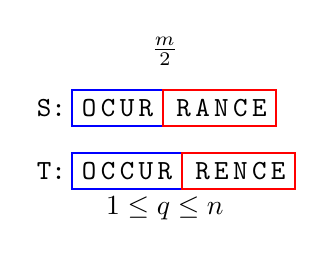
\begin{tikzpicture}[scale=0.8, auto,swap]
    % Draw a 7,11 network
    % First we draw the vertices


%case 1
   \def\d{0.3};
   \def\dx{0};
   \def\dy{0};

   \node[ultra thick] at (5*\d + \dx, \dy + 3* \d) {$\frac{m}{2}$} ;
    \foreach \i/\name/\id in {{-1/{S:}/}, {1/O\ /S1}, {2/C\ /}, {3/U\ /}, {4/R\ /S4}, {5/\ /}, {6/R\ /}, {7/A\ /}, {8/N\ /}, {9/C\ /SC}, {10/E\ /SE}}
        \node (\id) at (\i*\d + \dx,  \dy) {\tt \name };

   \def\dy{-1};
     \foreach \i/\name/\id in {{-1/{T:}/}, {1/O\ /T1}, {2/C\ /}, {3/C\ /}, {4/U\ /}, {5/R\ /T4}, {6/\ /}, {7/R\ /}, {8/E\ /}, {9/N\ /}, {10/C\ /TC}, {11/E\ /TE}}
        \node (\id) at (\i*\d + \dx,  \dy) {\tt \name };


    \draw[blue,  thick] (S1.south west) rectangle (S4.north east);
    \draw[blue,  thick] (T1.south west) rectangle (T4.north east);

    \draw[red,  thick] (S4.north east) rectangle (SE.south east);
     \draw[red,  thick] (T4.north east) rectangle (TE.south east);

    \node[ultra thick] at (5*\d + \dx, \dy - 2* \d) {$1\leq q \leq n$} ;

   \end{tikzpicture}
\end{figure}

我们有这个式子:
\begin{figure}[H]
\centering
\includegraphics[width=4.2in]{12.png}
\end{figure}
假设我们有了最优连配,其总体的分等于左一半的分和右一半的分相加;我们假设知道前一半是$align$ 到具体的哪个$q$那么就可以直接算。假如我们知道$q$,那么一切都有了,那么$q$到底是什么?

\subsection{算法}
我们来看这个算法

\sc Linear\_Space\_Alignment( S, T )
\begin{algorithmic}[1]
\STATE Allocate two arrays $f$ and $b$; each array has a size of $m$ .
\STATE {\sc Prefix\_Space\_Efficient\_Alignment}$( S, T[1..\frac{n}{2}], f)$;
\STATE {\sc Suffix\_Space\_Efficient\_Alignment}$( S, T[\frac{n}{2}+1, n], b)$;
\STATE Let $q^* = argmax_q ( f[q] + b[q] )$;
\STATE Free arrays $f$ and $b$;
\STATE Record $<q^*, \frac{n}{2}>$ in array $A$;
\STATE {\sc Linear\_Space\_Alignment}$( S[1..q^*], T[1..\frac{n}{2}] )$;
\STATE {\sc Linear\_Space\_Alignment}$( S[q^*+1..n], T[\frac{n}{2}+1, n] )$;
\RETURN $A$;
\end{algorithmic}

我们先申请两个数组,一个是$f$,一个是$b$。$f$代表前向数组,$b$代表后向数组。首先对S的左一半和T 整体进行$align$,结果放到$f $中,S的右一半和T进行$align$,结果放到$b$中。S的一半,$align$到T 的那个$q$呢?我们发现$q$是把$f$和$b$加起来,之间最大的那个数的位置。
\begin{figure}[H]
\centering
\includegraphics[width=3.2in]{13.png}
\end{figure}

S的左一半和T的OCCUR部分做$align$,也即我们想敲T的occur字符是敲成了OCUR这样。在上面的算法中,我们知道了$q*$,记录S<$q$,$n$/2>,表示$n$/2是从$q$这里变来的,剩下的我们递归调用即可。
\begin{figure}[H]
\centering
\includegraphics[width=3.2in]{14.png}
\end{figure}
\subsection{算法总结}
这样的话这个算法的思想分为三点:

    1.只用两个数组就可以得到最后的分数。

    2.可以从前往后算也可以从后往前算,最终结果是一样的。

    3.假设知道了最优的连配,那么S的左一半和右一半是从哪里得来的呢?我们假设这个位置是$q$,并且提供了定位的方法。

这个算法声称解决了动态规划的空间消耗问题,其使用了O($m$+$n$)的空间。

那么这个算法会不会增加了时间?过去的算法是O($m$*$n$),这是因为$m$*$n$个单元,每个单元是从三个数中取最大,每个要进行三次比较所以是3$m$$n$。这个新算法还是O($m$*$n$)的时间,怎么证明?这个超过了第一堂课递归主定理的范畴,因为这里的递归调用依赖于S的左一半和T的前一半,前一半到哪里不能事先知道。那应该怎么办?我们采用连蒙带猜的方法,猜并且带入验证。
我们设T($m$,$n$)是O($m$$n$)的时间,首先假设$m$'<$m$ $n$'<$n$

则$T(m',n') \leq km'n'$ 对于任意的 $m'<m$ and $n'<n$ 成立.故而有以下证明:
\begin{eqnarray}
 T(m,n) & = & cm +  T(q, \frac{n}{2}) + T(m-q, \frac{n}{2})  \\
      &\leq &  cm +  k q  \frac{n}{2} + k (m-q) \frac{n}{2}  \\
      &=& cm +  k q  \frac{n}{2} + k m \frac{n}{2} - k q \frac{n}{2}  \\
      &\leq& (c + \frac{k}{2}) mn  \\
      &=& kmn  \qquad \qquad  (set\ k=2c)
\end{eqnarray}

这个递归的证明和分治的时候不同,每个子问题的大小,即$q$的大小不知道,以后类似的问题可以这么做。另外,我们通过这个例子知道知道动态规划的内存是可以降下来的。

\section{alignment 问题的四个扩展}
\subsection{第一个扩展}
关于这个联配问题,有四个扩展,第一点是全局的连配到局部的连配,全局的连配是两个单词进行连配,但是这个是不够的。之前的算法只适合单词改错,不适合判断抄袭。比如说我只有一道题是抄的,其他部分我都很老实,这样总体的分还是比较低。只关心其中部分的分,就是局部的连配。这是Smith-Waterman 在1981 年做的工作。

局部的连配公式和原来的区别在于在原来的基础上加了0,也就是一旦也就是罚的分够狠,小于0,就重新从0开始。以前的分是指总体的S来自于T的概率,由于抄袭只有一部分,应该只关心一部分的分。

局部连配公式:

$d( S, T) = \max  \left \{ \begin{array}{ll}  \delta(S_n, T_n) + d(S[1..n-1], T[1..n-1]) &  \\
  \delta(`\_', T_n) + d(S, T[1..n-1]) & \\
  0 &\\
 \delta(S_n,`\_') + d(S[1..n-1],T) &  \end{array}
 \right. $

全局连配的公式:

$d( S, T) = \max  \left \{ \begin{array}{ll}  \delta(S_n, T_n) + d(S[1..n-1], T[1..n-1]) &  \\
  \delta(`\_', T_n) + d(S, T[1..n-1]) & \\
 \delta(S_n,`\_') + d(S[1..n-1],T) &  \end{array}
 \right. $

\subsection{第二个扩展}
上次说的罚分,实际使用的时候,如果$match$ +1,如果是插入 -3, 删除 -3,$mismatch$ -1。上堂课我们讲为什么不是扣3.1415926分,这是大家需要考虑的。实际工作中会用下面这个表格,一个字母变成另外一个字母的分是通过概率统计出来的,如A变成R表示-2 分。这些是怎么来的呢?我们统计这样一个概率:P (‘A’$|$'A'),然取$log$,然后取整,就是这个表格里的数。如果我们做的算法不结合统计,是得不到好的效果的。

\begin{figure}[H]
\centering
\includegraphics[width=3.3in]{L6-PAM.png}
\end{figure}

\subsection{第三个扩展}
刚才的例子,得到的分数是4,4分是高还是低,如何评判分高和低?我们提出P (S,T$|$Random),即想写T的时候,写成S的概率有多大。
我们有这样的计算公式:

分数大于$S$的概率是 $1-e^{-y}$, 其中 $y=K m n e^{-\lambda S}$.
具体可以参考论文。

\subsection{第四个扩展}
最后一个扩展是我的工作:
这个连配的算法非常简单,只是三个数求MAX,不需要用CPU来算,并且可以同时算有并行性。所以做了一个FPGA 的卡来实现这个算法,从图中可以看出,对于1000k的字符串,一个卡能顶1000 多个cpu,以后当我们从算法设计的角度无法提高性能的时候,可以考虑这种方法。
\begin{figure}[H]
\centering
\includegraphics[width=3in]{L6-PE.png}
\end{figure}
\begin{figure}[H]
\centering
\includegraphics[width=3in]{L6-MatrixCard.png}
\end{figure}
\begin{figure}[H]
\centering
\includegraphics[width=3in]{L6-FPGA-Speedup.png}
\end{figure}


\section{图上递归问题}
我们对数据结构进行分类

第一类是$sequences$(数组),比如第一堂课讲的n个数排序,可以分成左一半,右一半。

第二类是$graph$(图),图的特例是树,图的递归的例子是旅行商问题。

第三类是$set$(集合)。总体上来看,我们在这三种数据结构上进行递归,我们接下来讲图上递归的问题。

\subsection{TSP问题}
TSP是一个图上递归的例子:我们来回顾一下TSP问题。
\begin{figure}[H]
\centering
	\begin{tikzpicture}[scale=1, auto,swap]

    \foreach \pos/ \name in {{(0,0)/1},{(0,2)/2}, {(2,2)/3}, {(2,0)/4}}
        \node[smallvertex,fill=blue!20] (\name) at \pos{$\name$};


    % Connect vertices with edges and draw weights
    \foreach \source/ \dest/\weight in {2/1/{1},   1/4/{3}, 3/2/{5}, 4/3/{3}}
        \path[undirectededge] (\source) -- node[weight] {$\weight$} (\dest);
    \foreach \source/ \dest/\weight in  {3/1/{8}, 4/2/{7}}
        \path[undirectededge] (\source) -- node[weight] {$\weight$} (\dest);

	\end{tikzpicture}
\end{figure}

给定图,从1号节点,经过所有节点回到1,找路径最短。假设了从1号节点出发。要考虑这个问题,只要考虑一个跟它相关的问题:我们定义D(S,$e$,这是一个子问题,表示我们从1出发,旅行过S中所有的节点,到达$e$距离最短,这个距离是D(S,$e$。为什么要解决这个子问题?因为只要解决了这个子问题,就能解决前面的问题:因为我们是想从1出发,经过所有城市,最后回到1。那么是从哪里回来的?可能是2 3 4。最后的旅程可以这么表示:

$\min\{ D( \{2, 3, 4\}, 2)  + d_{2,1}$, \\$ D( \{2, 3, 4\}, 3 ) + d_{3,1},$ \\ $D( \{2, 3, 4\}, 4 ) + d_{4,1} \}$

但是这个要怎么算?我们还是老的套路,先从最简单的例子来看,如果S只包含一个或者两个城市,会不会很简单?我们在这种情况下求最小就可以了。怎么做呢?

\begin{figure}[H]
\centering
	\begin{tikzpicture}[scale=1, auto,swap]

    \foreach \pos/ \name in {{(0,0)/1},{(0,1.5)/2}, {(2,1.5)/3}}
        \node[smallvertex,fill=blue!20] (\name) at \pos{$\name$};

    % Connect vertices with edges and draw weights
    \foreach \source/ \dest/\weight in {2/1/{1},   3/2/{5}}
        \path[undirectededge] (\source) -- node[weight] {$\weight$} (\dest);
    \foreach \source/ \dest/\weight in  {3/1/{8}}
        \path[undirectededge] (\source) -- node[weight] {$\weight$} (\dest);

    \foreach \source/ \dest/\weight in {2/1/{},   3/2/{}}
        \path[undirectededge, red] (\source) -- node[weight] {$\weight$} (\dest);

    \foreach \pos/ \name in {{(3,0)/1},{(3,1.5)/2}, {(5,1.5)/3}}
        \node[smallvertex,fill=blue!20] (\name) at \pos{$\name$};

    % Connect vertices with edges and draw weights
    \foreach \source/ \dest/\weight in {2/1/{1},   3/2/{5}}
        \path[undirectededge] (\source) -- node[weight] {$\weight$} (\dest);
    \foreach \source/ \dest/\weight in  {3/1/{8}}
        \path[undirectededge] (\source) -- node[weight] {$\weight$} (\dest);

    \foreach \source/ \dest/\weight in {2/3/{},   3/1/{}}
        \path[undirectededge, red] (\source) -- node[weight] {$\weight$} (\dest);

	\end{tikzpicture}

\end{figure}
我们有如下结论:

$D( \{ 2\}, 2) = d_{12}$;
$D( \{ 3\}, 3) = d_{13}$;

这个是显然的; D{2}表示经过S中的所有节点一次,最后到达2。我们能解决简单的问题以后,复杂的问题该怎么办?比如$D(\{1,2, 3, 4\}, 4)$?

这里最终到达4,要么从2号来,要么从3号来, 我们有了最优子结构的式子:
 \begin{figure}[H]
 \centering
	\begin{tikzpicture}[scale=1, auto,swap]

    \foreach \pos/ \name in {{(0,0)/1},{(0,1.5)/2}, {(1.5,1.5)/3}, {(1.5,0)/4}}
        \node[smallvertex,fill=blue!20] (\name) at \pos{$\name$};


    % Connect vertices with edges and draw weights
    \foreach \source/ \dest/\weight in {2/1/{1},   1/4/{3}, 3/2/{5}, 4/3/{3}}
        \path[undirectededge] (\source) -- node[weight] {$\weight$} (\dest);
    \foreach \source/ \dest/\weight in  {3/1/{8}, 4/2/{7}}
        \path[undirectededge] (\source) -- node[weight] {$\weight$} (\dest);

%red 	
    \foreach \source/ \dest/\weight in  {1/2/{}, 2/3/{}, 4/3/{}}
        \path[undirectededge,red] (\source) -- node[weight] {$\weight$} (\dest);




    \foreach \pos/ \name in {{(3,0)/1},{(3,1.5)/2}, {(4.5,1.5)/3}, {(4.5,0)/4}}
        \node[smallvertex,fill=blue!20] (\name) at \pos{$\name$};


    % Connect vertices with edges and draw weights
    \foreach \source/ \dest/\weight in {2/1/{1},   1/4/{3}, 3/2/{5}, 4/3/{3}}
        \path[undirectededge] (\source) -- node[weight] {$\weight$} (\dest);
    \foreach \source/ \dest/\weight in  {3/1/{8}, 4/2/{7}}
        \path[undirectededge] (\source) -- node[weight] {$\weight$} (\dest);

%red 	
    \foreach \source/ \dest/\weight in  {1/3/{}, 2/3/{}, 4/2/{}}
        \path[undirectededge,red] (\source) -- node[weight] {$\weight$} (\dest);


	\end{tikzpicture}
\end{figure}
	\begin{itemize}
		\item $D( \{1, 2, 3, 4\}, 4) = \min\{ D( \{1, 2, 3\}, 3) + d_{34}, D( \{1, 2, 3\}, 2) + d_{24} \} $;
		\item 最优子结构性质: \\$D(S, e) = \begin{cases}		
										d_{1e} & \text{ if } S=\{e\} \\
										\min_{m\in{S-\{e\}}} (D(S-\{e\}, m) + d_{me})& \text{otherwise}
										\end{cases}$
	\end{itemize}

有了这个递归表达式,就可以写一个算法如下:

\bf function $D(S, e)$
\begin{algorithmic}[1]
\IF{ $S = \{ e \}$}
	\RETURN{ $d_{1e}$};	
\ENDIF	
\STATE $d = \infty$;
\FORALL{ city $m \in S$, and $m \neq e$ }
	\IF{ $D( S - \{e\}, m) + d_{me} < d $ }
		\STATE $d = D( S - \{e\}, m) + d_{me}$;
	\ENDIF
\ENDFOR
\RETURN{$d$};
\end{algorithmic}


 这是图上递归的例子,我原来是4个节点的图G,通过递归把图变小了。过去的递归都是在数组上比较好理解,现在是一个图,对于一个四个节点的图不会做,可以变成三个节点...但是这个算法性能不怎么好。这个算法的时间复杂度和空间复杂度如下:
\begin{itemize}
	\item 空间复杂度:  $\sum_{k=2}^{n-1}  k {n-1 \choose k} + n-1= (n-1) 2^{n-2}$
	\item 时间复杂度:  $\sum_{k=2}^{n-1} k(k-1){n-1 \choose k} + n-1 = O( 2^n n^2)$.
\end{itemize}

我们先说空间复杂度:我们要枚举所有的子图,它有多少个呢?我们有D(S,e),s属于{1,2,$...$n},

e=1,2,3$...$;我们考虑子图规模为k,k取1到n-1。对于规模为k 的子图,其有k个子问题。我们最终算出来是2的n次方这个量级。中间的每个子问题都要存下来。那么时间复杂度呢?对于动态规划的算法的时间复杂度,我们看有多少个子问题,以及每个子问题要做多少次运算。由于我们要对all city求最小,所以我们在时间复杂度的式子基础上乘k-1,结果是$O( 2^n n^2)$。

\subsection{单源最短路问题}
我们接着往下看,还是在图上做递归的改进方法:单源最短路问题,它加了一点东西做改进。

\begin{figure}[H]
\centering
\includegraphics[width=2.2in]{sp.png}
\end{figure}

我们想求从S到T的最短路径,这个问题和TSP的不同在于不需要每个城市都走到(假设没有负圈)。我们先来尝试定义子问题。
\begin{itemize}
    \item 从S到T的路径,我们把这个过程看成一系列的决策,在每一个决策步考虑下一步往哪里走。
    \item 假如已经拿到了最优解O,考察O中的第一个决策:所有s的邻居都是可选项,这样选择了从s 到v的一条路。
    \item 剩下的问题是,从v中怎么达到t,路径越短越好;
\end{itemize}
这样,图变小了,定义了子问题。

但是按照这个递归表达式写程序有点慢,因为子问题的数量太多了,图上的递归,是指数级的,跟前面的问题遇到了相同的困难。所以我们做动态规划的时候要注意,有的时候定义的子问题不是特别合适,导致子问题数目为指数级。我们做了如下改进:

引入了新的观察,因为图中没有负圈,从S到T最短路最多只有n个节点。假设我们拿到了最优解O,考虑O 中的第一个决策。所有和s直连的点都有可能。当决定了第一步以后,问题变成从v到t 的最短路最多经过n-2 条边。从而我们修改了子问题,写出了最优子结构:

 \begin{small} $OPT[v, t,  k] = \min \begin{cases}
		OPT[ v, t,  k-1 ], \\
		\min_{<v,w>\in E} \{OPT[ w, t,  k-1 ] + d(v, w) \}
		\end{cases}$
		\end{small}

由于上面定义的是最多k条边,那么可能只走了k-1条边,k-2条边$...$,所以有了上面那一项。


算法如下
\sc Bellman\_Ford$( G, s, t )$
\begin{algorithmic}[1]
\FOR {any node $v\in V$  }
\STATE $OPT[v, t, 0] = \infty;$
\ENDFOR
\FOR{ $k=0$ to $n-1$ }
\STATE $OPT[t, t, k] = 0;$
\ENDFOR
\FOR{ $k=1$ to $n-1$ }
\FORALL{ node $v$ (in an arbitrary order) }
\STATE \begin{small} $OPT[v, t, k] = \min \begin{cases}
		OPT[v, t, k-1 ]\\
		\min_{<v,w>\in E} \{OPT[w, t,  k-1 ] + d(v,w) \}
		\end{cases}$
		\end{small}
\ENDFOR
\ENDFOR
\RETURN {$OPT[s, t, n-1]$};
\end{algorithmic}
我们仔细看一下这个算法:我们先看第7行到第10行,第9行是我们的递归表达式。初始化阶段,v到t经过0 步无法到达,所以设置无穷。自己到自己,无论经过几步,都是0。

”$Richard Bellman on the birth of dynamic programming$” (S.Dreyfus, 2002)大家有时间可以看一下这篇$paper$,对理解动态规划很有帮助。

我们看一个例子,对这么一个道路交通网络,我们问到达$t$的最短路径是什么。
\begin{figure}[H]
\centering
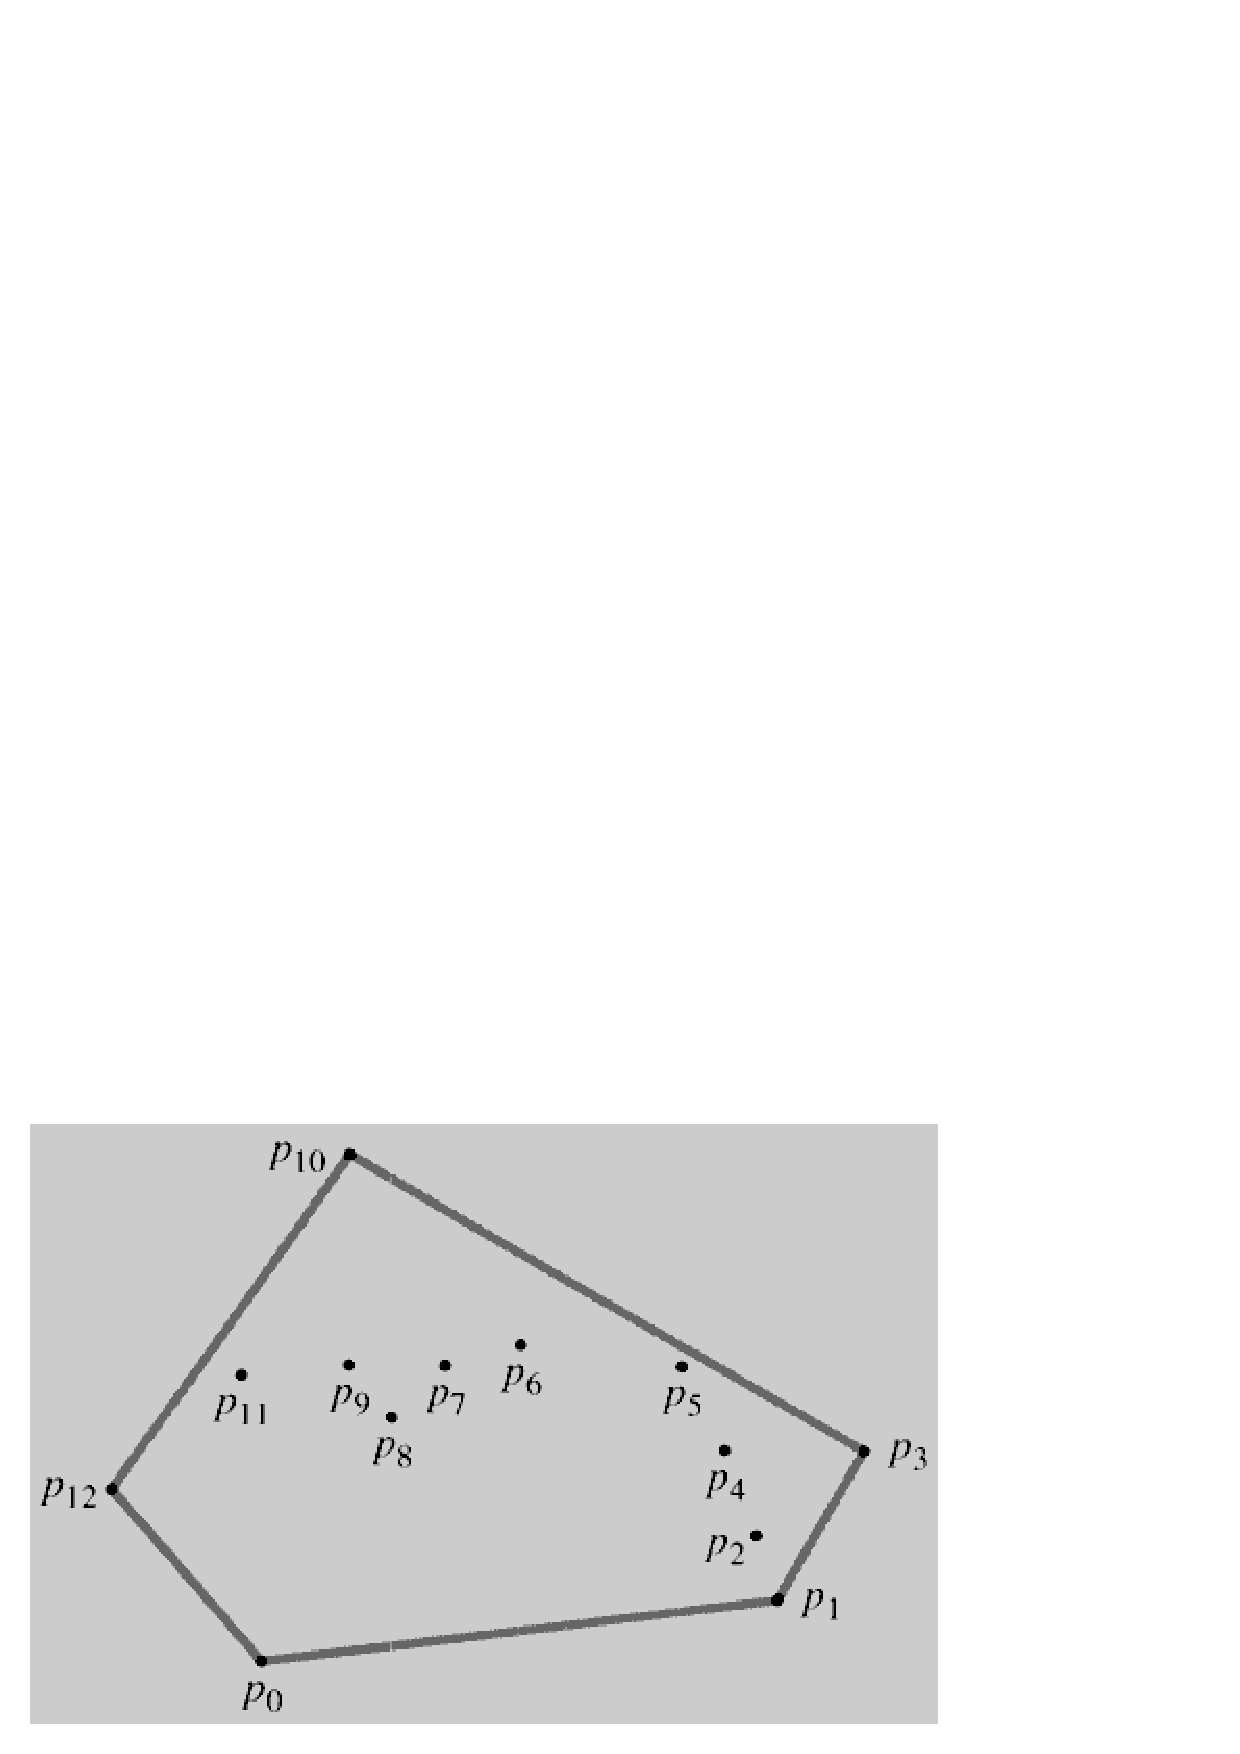
\includegraphics[width=4.2in]{example.png}
\end{figure}

我们的子问题是,从任意一个节点出发,经过$k$步到达$t$的路程这样我们有了第一行和第一列。我们发现$a$到$t$可以直达,所以表格的(1,1) = -3;这个可以解释为OPT($a$,$t$,1)=$min${OPT($a$,$t$,0), OPT($w$,$t$,0)+$d${$aw$}} 这里的$w$=$t$,剩下的部分以此类推。


\begin{figure}[H]
\centering
\includegraphics[width=4.2in]{tree.png}
\end{figure}
这幅图给大家扩展一个小知识,我们发现把所有的点到达$t$的最短路径都画出来,他们不会一个复杂的图,是一个$tree$,这个将来会有用。

\subsection{负圈判断问题}
如果$v$可以到达$t$,从$v$到$t$有负圈,那么我么有这个式子: $\lim_{k \rightarrow \infty} OPT(  v, t, k ) = - \infty $。
$k$越来越大,它会越来越小。我们给出下面这样一个图:
\begin{table}[H]
\begin{tabular}{|r|r|r|r|r|r|r|r|r|r|r|r|r|}
\hline
源点   & k=0  & k=1 & k=2 & k=3 & k=4 & k=5 & k=6 & k=7 & k=8 & k=9 &k=10& k=11 \\ \hline
$t$ & 0 & 0 & 0 & 0 & 0 & 0 & 0 & 0 & 0 & 0 & 0 & 0\\ \hline
$a$ & - & -3 & -3 & -4 & -6 & -6 & -6 &-6  & -6 & -6 & -6 & -6 \\ \hline
$b$ & - & - & 0 & -2 & -2 & -2 & -2 & -2 & -2 & -2 & -2 & -2 \\ \hline
$c$ & - & 3 & 3 & 3 & 3 & 3 &  3&  3&  3&  3&  3&  3\\ \hline
$d$ & - & 4 & 3 & 3 & 2 & 0 &  0 & 0  & 0  & 0  & 0  & 0  \\ \hline
$e$ & - & 2 & 0 & 0 & 0 & 0 &  0 &  0 & 0  & 0  &  0 &  0 \\ \hline
\end{tabular}
\end{table}

所以出现了图的负圈判断问题。
如果里面没有负圈,我们可以得到这样一个结论:对于$k$>$n$,结果是一样的。我们回到一个有负圈的图,如果我接着计算下去,可以发现值越来越小。所以判断有没有负圈,只要把这个$Bellman$$-$$Ford$算法多跑几次就可以。多跑几次,可以看到周期是2,所以圈是三个节点。任意给我们一个图,问里面有没有负圈,应该怎么办?我们可以把这个图做一个扩展,加入一个节点,然所有的节点都指向它,边长为0。然后我们运行上面的算法,如果有负圈,到$t$的最短路径会越来越小,这就是负圈的判断方法。

说到最短路径,大家第一个想到$dijkstra$。这个算法有了,为什么还要用$Bellman$$-$$Ford$? 我们来看算法在路由器上面的应用:有一个复杂的网络的图,中间每个节点是一个$router$,我们如果在网络中找到$google$的最短路径我们如果用$dijkstra$算法,会有问题。找最短路径需要全局信息,但是这个信息是拿不到的。而$Bellman$$-$$Ford$算法只要知道local的信息就可以了。

下面是每台路由器上跑的程序,一开始是每台路由器只能自己到自己。任何一个路由器$w$,发现到达$google$有条近路,我就把这个消息告诉所有的邻居。我就把邻居$w$到$google$的距离+我到$w$的距离,和我过去到达$google$要花的时间求最小,并且更新。这里,任意一个路由器发现了最短路,只要告诉邻居就够了,从来不需要关心整个$internet$。

\sc AsynchronousShortestPath$( G, s, t )$
\begin{algorithmic}[1]
\STATE Initially, set $OPT[t, t]=0$, and $OPT[v, t]=\infty$;
\STATE Label node $t$ as ``active'';
\WHILE{ exists an active node}
\STATE arbitrarily select an active node $w$;
\STATE remove $w$'s active label;
\FORALL{ edges  $<v, w>$ (in an arbitrary order) }
\STATE $OPT[v, t] = \min \begin{cases} OPT[v, t] \\ OPT[w, t]+ d(v,w) \end{cases}$
\IF{ $OPT[v, t]$ was updated }
\STATE label $v$ as "active";
\ENDIF
\ENDFOR
\ENDWHILE
\end{algorithmic}
接着我们来看一个相关的问题,最长路径问题。这个问题和最短路径问题对应,需要找从源点到目标节点的最长路径。这是一个NP难问题,非常非常难。动态规划的$Bellman$$-$$Ford$方法在这里不行,因为这个问题不好分。假设把从$q$到$t$的问题变成两个问题$q$到$r$和$r$到$t$:
\begin{enumerate}
\item
 $P(q, r) = q\rightarrow s \rightarrow t\rightarrow r$
\item
 $P(r, t) = r \rightarrow q \rightarrow s \rightarrow t$,
\end{enumerate}

我们可能得到的解是: $q\rightarrow s \rightarrow t\rightarrow r \rightarrow q \rightarrow s \rightarrow t$, 这不是简单路径。

在最长路径问题中,不能分解因为两个子问题可能有联系。在最短路径问题中就不会遇到这个问题。如果把最短路径问题分解成两个子问题,假设两个子问题$q$ 到$r$和$r$到$t$之间有共享一个点$w$,那么就会形成一个圈,把这个圈去掉以后会得到一个更短的路径,因为我们假设了没有负圈。

\section{下节课内容}
我们在讲动态规划的时候,分解子问题,由于不知道要怎么分,所以需要枚举。如果我们加入一点更严的限制的话,我们就不用枚举了。分治的时候,我们就这么分,不用枚举。动态规划的时候,我们不知道怎么分,所以要枚举。如果我们的问题更特殊一点,就不用枚举了,直接就知道选谁。这是什么算法呢?这就是贪心算法。它是动态规划算法的一个加强的版本。我们在$Bellman-Ford$算法中用到枚举,如果我们加一个条件,我们就知道下家走谁,根本就不用枚举,这就是$Dijkstra$算法。

